%!TEX program = xelatex
\let\stop\empty

\documentclass[12pt,a4paper,fontset=none]{exam-zh}
% ==========================
% 卷面变量设置（只需改这里）
% ==========================
\newcommand{\paperlevel}{初中一}
\newcommand{\papersubject}{数学 试卷一}
\newcommand{\schoolname}{金宝培元独立中学}
\newcommand{\examname}{年终考}
\newcommand{\classinfo}{J1(H / I/ F)}
\newcommand{\examdate}{30-10-2026}
\newcommand{\examtime}{12:15-13:00}
\newcommand{\questiontotal}{20}
\newcommand{\paperpercentage}{40\%}
\newcommand{\setterteacher}{蔡杰庆师}
\newcommand{\reviewteacher}{禤佩娟师}
\newcommand{\secondreviewteacher}{张惠雯师}
\newcommand{\auditteacher}{雷泳健师}



\usepackage{xeCJK}
\setCJKmainfont{NSimSun}
\newCJKfontfamily\heiti{NSimSun}
\usepackage{geometry}
\usepackage{array}
\usepackage{tikz}
\usetikzlibrary{calc,angles,quotes}
\usepackage{amsmath}
\usepackage{wrapfig}
\usepackage{adjustbox}
\usepackage{enumitem}
\usepackage{fancyhdr}
\usepackage{scalerel}
\providecommand{\wideparen}[1]{\overset{\frown}{#1}}
\def\mcirc{\mathbin{\scalerel*{\circ}{j}}}
\def\msquare{\mathord{\scalerel*{\Box}{gX}}}
\geometry{margin=2cm}

% \AtBeginDocument{\zihao{4}}
% ----------- 调整 exam -----------


% --- 全局样式定义 ---
% 定义选择题环境：题号 1. 2.，选项 A. B. C. D. 粗体，且保留 1.5em 间距
\examsetup{
    page = {
    size = a4paper,           % 设定纸张大小 [4]
    foot-content = { - ; - }  % 页脚显示为 -1-, -2- 格式 [3]
  },
    choices = {
    label-pos = top-left,
    column-sep = 1em,
    label-pos = auto,
    label-sep = 0.5em,
    max-columns = 4
    },
  question = {
    top-sep    = 1em, % 调整题目上方的垂直距离（默认值为 .5em plus .5em minus .2em）
    bottom-sep = 1em  % 调整题目下方的垂直距离（默认值为 .5em plus .5em minus .2em）
  },
    paren = {
    show-paren = false  % 设置为 false 则不显示括号 [3, 4]
  },
    choices = {
    label = \textbf{\Alph*}
  }, 
    solution = {
    show-solution = hide, % 隐藏解答
    label-content = {参考答案},  % 答案区的标题文字
    show-qed = true            % 在解答末尾显示结束符号 ◻ 
  }
}



\makeatletter
\newcounter{answerkeyquestion}
\let\answerkeytotal\questiontotal
\let\originalparen\paren
\newcommand{\answerkeyitems}{}
\newcommand{\addanswerkeyitem}[2]{%
  \pgfmathtruncatemacro{\row}{ifthenelse(#1<=\cols,0,1)}%
  \pgfmathtruncatemacro{\col}{mod(#1-1,\cols)}%
  \pgfmathsetlengthmacro{\x}{\col*\boxw}%
  \pgfmathsetlengthmacro{\y}{-\row*\boxh}%
  \draw (\x,\y) rectangle ++(\boxw,\boxh);%
  \node[anchor=north west] at (\x+\offset,\y+\boxh-\offset) {\textbf{#1.}};%
  \node at (\x+0.6*\boxw,\y+0.45*\boxh) {\Large\textbf{#2}};%
}
\renewcommand{\paren}[1][]{%
  \originalparen[#1]%
  \edef\answerkeytemp{#1}%
  \ifx\answerkeytemp\@empty\else
    \stepcounter{answerkeyquestion}%
    \begingroup
      \edef\x{\endgroup
        \noexpand\g@addto@macro\noexpand\answerkeyitems{\noexpand\addanswerkeyitem{\theanswerkeyquestion}{#1}}}%
    \x
  \fi
}
\makeatother

\newcommand{\makeexamheader}{%
% ==========================
% 三栏标题区
% ==========================
\noindent
\begin{tabular*}{\textwidth}{@{\extracolsep{\fill}} p{0.3\textwidth} p{0.35\textwidth} p{0.3\textwidth}}

\raggedright
\textbf{\paperlevel}\\[0.2em]
\textbf{}{\papersubject}\\[0.4em]
姓名：\underline{\hspace{3cm}} &

\centering
\textbf{\schoolname}\\[0.2em]
\textbf{\examname}\\[0.4em]
班级：\classinfo&

\raggedright
日期：\examdate\\[0.2em]
时间：\examtime\\[0.4em]
得分：\underline{\hspace{2.5cm}} \\

\end{tabular*}

\begin{flushleft}
考生须知： 
选出正确的答案，用蓝或黑色的原子笔将答案的相应选项字母填入本页特备作答栏。
\end{flushleft}

% =========================
% 答题栏
% =========================
\begin{flushleft}
\textbf{特备答题栏:}
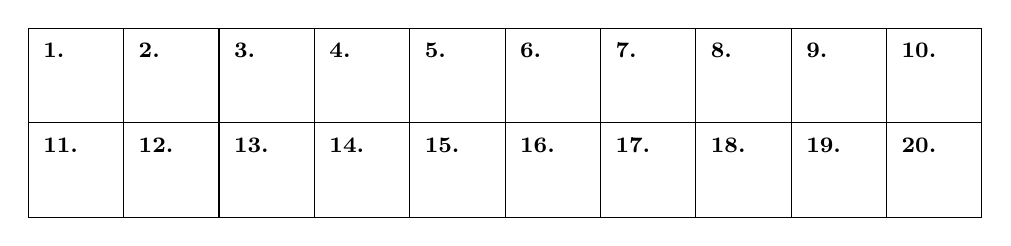
\begin{tikzpicture}
  % ---- 根据题数自动设置：16题为 8×2，20题为 10×2 ----
  \pgfmathtruncatemacro{\cols}{ifthenelse(\answerkeytotal<=16,8,10)}
  \pgfmathsetlengthmacro{\boxw}{(\linewidth-0.4pt)/\cols}
  \pgfmathsetlengthmacro{\boxh}{1.2cm}
  \pgfmathsetlengthmacro{\offset}{0.15cm}

  \foreach \num in {1,...,\answerkeytotal} {
    \pgfmathtruncatemacro{\row}{ifthenelse(\num<=\cols,0,1)}
    \pgfmathtruncatemacro{\col}{mod(\num-1,\cols)}
    \pgfmathsetlengthmacro{\x}{\col*\boxw}
    \pgfmathsetlengthmacro{\y}{-\row*\boxh}
    \draw (\x,\y) rectangle ++(\boxw,\boxh);
    \node[anchor=north west, font=\footnotesize, inner sep=1pt] at (\x+\offset,\y+\boxh-\offset) {\textbf{\num.}};
  }
\end{tikzpicture}

\end{flushleft}
}


\begin{document}
\makeexamheader

%region 范围：1–3 二八进制互换 | 考点：二进数加法、二进数转八进数（三位一组分组法） | 难度：易
\begin{question}
    已知二进数 $101101_2+11011_2=A_8$，则 $A=$ \paren[B]
    \begin{choices}
        \item $104$
        \item $110$
        \item $72$
        \item $440$
    \end{choices}
\end{question}

\begin{solution}
    求 $A$，使 $101101_2+11011_2=A_8$。 \\
    先在二进制中逐位相加，再从个位向左每三位一组，把和化为八进数。
    \begin{align*}
        101101_2+11011_2 &= 1001000_2 \\
        &= {\underline{001}\ \underline{001}\ \underline{000}}_2 \\
        &= {1\ 1\ 0}_8 \\
        A &= 110
    \end{align*}
    故选 B。
\end{solution}
%endregion

%region 范围：1–2 二进制与十进制互换 | 考点：不同进制数的大小比较（统一化为十进制） | 难度：易
\begin{question}
    已知 $10110_2<x<11110_2$，则下列哪一项是$x$ 的可能值 \paren[C]？
    \begin{choices}
        \item $10101_2$
        \item $11111_2$
        \item $27_8$
        \item $36_8$
    \end{choices}
\end{question}

\begin{solution}
    已知 $10110_2<x<11110_2$，判断哪个选项可能是 $x$。 \\
    各数进制不同，统一化为十进制后再比较大小。
    \begin{align*}
        10110_2 &= 1\times2^4+0\times2^3+1\times2^2+1\times2+0 = 22 \\
        11110_2 &= 1\times2^4+1\times2^3+1\times2^2+1\times2+0 = 30 \\
        10101_2 &= 16+4+1 = 21 \\
        11111_2 &= 16+8+4+2+1 = 31 \\
        27_8 &= 2\times8+7 = 23 \\
        36_8 &= 3\times8+6 = 30
    \end{align*}
    由 $22<x<30$，只有 $23$ 满足。\\
    故选 C。
\end{solution}
%endregion

%region 范围：1–3 二八进制互换 | 考点：二、八进数互换结果的正误判断 | 难度：中
\begin{question}
    下列二进数与八进数的互相转换中，结果\textbf{正确}的是 \paren[B]？
    \begin{choices}
        \item $11010_2=31_8$
        \item $574_8=101111100_2$
        \item $1110101_2=724_8$
        \item $703_8=11100011_2$
    \end{choices}
\end{question}

\begin{solution}
    判断四个转换结果中哪一个正确。 \\
    逐项按三位一组（二$\to$八）或一位拆三位（八$\to$二）验算。
    \begin{align*}
        11010_2 &= {\underline{011}\ \underline{010}}_2 = 32_8 \neq 31_8 \\
        574_8 &= {\underline{101}\ \underline{111}\ \underline{100}}_2 = 101111100_2 \\
        1110101_2 &= {\underline{001}\ \underline{110}\ \underline{101}}_2 = 165_8 \neq 724_8 \\
        703_8 &= {\underline{111}\ \underline{000}\ \underline{011}}_2 = 111000011_2 \neq 11100011_2
    \end{align*}
    故选 B。
\end{solution}
%endregion

%region 范围：4–5 1.6.1 比与比例的概念及性质 | 考点：化简比（先统一单位，再化为整数比） | 难度：易
\begin{question}
    化简比 $\dfrac{2}{5}$ 小时 $:\ 1.5$ 分钟 \paren[C]。
    \begin{choices}
        \item $4:15$
        \item $8:5$
        \item $16:1$
        \item $80:3$
    \end{choices}
\end{question}

\begin{solution}
    化简比 $\dfrac{2}{5}$ 小时 $:\ 1.5$ 分钟。 \\
    两项单位不同，先把小时化为分钟，再同乘 $10$ 化为整数比。
    \begin{align*}
        \dfrac{2}{5}\text{ 小时} &= \dfrac{2}{5}\times 60 = 24\text{ 分钟} \\
        24:1.5 &= (24\times 10):(1.5\times 10) \\
        &= 240:15 \\
        &= 16:1
    \end{align*}
    故选 C。
\end{solution}
%endregion

%region 范围：6–7 1.6.2 连比 | 考点：化简比（小数比、分数比）、由 $x:y$ 与 $y:z$ 求 $x:z$ | 难度：中等
\begin{question}
    已知 $x:y=2.4:3.6$，$y:z=\dfrac{1}{5}:\dfrac{3}{10}$，则 $x:z=$ \paren[D]
    \begin{choices}
        \item $2:9$
        \item $2:3$
        \item $1:1$
        \item $4:9$
    \end{choices}
\end{question}

\begin{solution}
    由 $x:y=2.4:3.6$ 与 $y:z=\dfrac{1}{5}:\dfrac{3}{10}$ 求 $x:z$。 \\
    先把两个比各自化为最简整数比，再统一 $y$ 的份数，得到连比。
    \begin{align*}
        x:y &= 2.4:3.6 = (2.4\times 10):(3.6\times 10) = 24:36 = 2:3 \\
        y:z &= \dfrac{1}{5}:\dfrac{3}{10} = \left(\dfrac{1}{5}\times 10\right):\left(\dfrac{3}{10}\times 10\right) = 2:3 \\
        x:y &= 2:3 = (2\times 2):(3\times 2) = 4:6 \\
        y:z &= 2:3 = (2\times 3):(3\times 3) = 6:9 \\
        x:y:z &= 4:6:9 \\
        x:z &= 4:9
    \end{align*}
    故选 D。
\end{solution}
%endregion

%region 范围：6–7 1.6.2 连比 | 考点：由连比 $a:b:c$ 求相邻两项的比，再用比例基本性质求未知项 | 难度：易
\begin{question}
    已知 $a:b:c=6:8:10$，若 $a:b=2:m$，$b:c=4:n$，则 $m+n=$ \paren[B]
    \begin{choices}
        \item $\dfrac{13}{2}$
        \item $\dfrac{23}{3}$
        \item $\dfrac{26}{3}$
        \item $9$
    \end{choices}
\end{question}

\begin{solution}
    由 $a:b:c=6:8:10$ 及 $a:b=2:m$，$b:c=4:n$，求 $m+n$。 \\
    连比中相邻两项的比与已知比相等，分别用比例的基本性质求 $m$ 与 $n$。
    \begin{align*}
        a:b &= 6:8 = 2:m & b:c &= 8:10 = 4:n \\
        6m &= 8\times 2 & 8n &= 10\times 4 \\
        m &= \dfrac{8}{3} & n &= 5 \\
        m+n &= \dfrac{8}{3}+5 = \dfrac{23}{3}
    \end{align*}
    故选 B。
\end{solution}
%endregion

%region 范围：6–7 1.6.2 连比 | 考点：连比的求法及按连比分配 | 难度：中
\begin{question}
    甲、乙、丙三人共有 $620$ 元，已知甲与乙的钱之比为 $3:4$，乙与丙的钱之比为 $6:5$，则丙有多少元 \paren[B]？
    \begin{choices}
        \item $240$ 元
        \item $200$ 元
        \item $180$ 元
        \item $310$ 元
    \end{choices}
\end{question}

\begin{solution}
    求甲、乙、丙共有 $620$ 元时丙的钱数。 \\
    先由两个比求出甲、乙、丙的连比，再按总份数分配。
    \begin{align*}
        \text{甲}:\text{乙} &= 3:4 = 9:12 \\
        \text{乙}:\text{丙} &= 6:5 = 12:10 \\
        \text{甲}:\text{乙}:\text{丙} &= 9:12:10 \\
        \text{丙} &= 620\times\dfrac{10}{9+12+10} \\
        &= 620\times\dfrac{10}{31} \\
        &= 200\ (\text{元})
    \end{align*}
    故选 B。
\end{solution}
%endregion

%region 范围：8–10 1.6.3 正、反比例及比例分配 | 考点：正比例关系的应用 | 难度：易
\begin{question}
    同一时刻，同一地点，物体的高度与它的影长成正比例。已知一根高 $6$ 米的竹竿的影长为 $4$ 米，此时旁边一棵树的影长为 $10$ 米，则这棵树的高度为 \paren[C]？
    \begin{choices}
        \item $12$ 米
        \item $2.4$ 米
        \item $15$ 米
        \item $\dfrac{20}{3}$ 米
    \end{choices}
\end{question}

\begin{solution}
    求影长为 $10$ 米的树的高度。 \\
    高度与影长成正比例，对应的高度与影长之比相等。 \\
    设树高 $x$ 米。
    \begin{align*}
        \dfrac{x}{10} &= \dfrac{6}{4} \\
        4x &= 6\times 10 \\
        x &= 15
    \end{align*}
    故选 C。
\end{solution}
%endregion

%region 范围：8–10 1.6.3 正、反比例及比例分配 | 考点：反比例关系的应用 | 难度：中
\begin{question}
    某水池需要抽干积水，用 $6$ 台相同的水泵同时工作，$10$ 小时可以抽完。若要求 $4$ 小时抽完，则至少需要多少台水泵 \paren[B]？
    \begin{choices}
        \item $12$ 台
        \item $15$ 台
        \item $24$ 台
        \item $60$ 台
    \end{choices}
\end{question}

\begin{solution}
    求 $4$ 小时抽完积水所需的水泵台数。 \\
    积水总量一定，台数与时间成反比例，即台数与时间之积为定值。 \\
    设需要 $x$ 台。
    \begin{align*}
        4x &= 6\times 10 \\
        4x &= 60 \\
        x &= 15
    \end{align*}
    故选 B。
\end{solution}
%endregion

%region 范围：8–10 1.6.3 正、反比例及比例分配 | 考点：简单比例分配 | 难度：中
\begin{question}
    把 $780$ 元按 $\dfrac{1}{2}:\dfrac{1}{3}:\dfrac{1}{4}$ 的比分给甲、乙、丙三人，则甲分得的钱数为 \paren[B]？
    \begin{choices}
        \item $390$ 元
        \item $360$ 元
        \item $240$ 元
        \item $180$ 元
    \end{choices}
\end{question}

\begin{solution}
    求按 $\dfrac{1}{2}:\dfrac{1}{3}:\dfrac{1}{4}$ 分配 $780$ 元时甲分得的钱数。 \\
    先将连比化为整数比，再按总份数分配。
    \begin{align*}
        \dfrac{1}{2}:\dfrac{1}{3}:\dfrac{1}{4} &= \left(\dfrac{1}{2}\times 12\right):\left(\dfrac{1}{3}\times 12\right):\left(\dfrac{1}{4}\times 12\right) = 6:4:3 \\
        \text{甲分得} &= 780\times\dfrac{6}{6+4+3} \\
        &= 780\times\dfrac{6}{13} \\
        &= 360\ (\text{元})
    \end{align*}
    故选 B。
\end{solution}
%endregion

%region 范围：11–12 2.1.1 代数式及代入求值 | 考点：列代数式 | 难度：易
\begin{question}
    小明买了 $3$ 支单价为 $a$ 元的笔和 $2$ 本单价为 $b$ 元的本子，付给店员 $50$ 元，则应找回多少元 \paren[D]？
    \begin{choices}
        \item $3a+2b-50$
        \item $50-2a-3b$
        \item $50-5(a+b)$
        \item $50-3a-2b$
    \end{choices}
\end{question}

\begin{solution}
    求付 $50$ 元后应找回的钱数。 \\
    找回的钱数等于付款数减去所花的总钱数。
    \begin{align*}
        \text{所花总钱数} &= 3a+2b \\
        \text{找回} &= 50-(3a+2b) \\
        &= 50-3a-2b
    \end{align*}
    故选 D。
\end{solution}
%endregion

%region 范围：11–12 2.1.1 代数式及代入求值 | 考点：代数式代入求值（含负数） | 难度：中
\begin{question}
    当 $a=-2$，$b=3$ 时，代数式 $2a^2-3ab+b^2$ 的值为何 \paren[B]？
    \begin{choices}
        \item $-1$
        \item $35$
        \item $19$
        \item $43$
    \end{choices}
\end{question}

\begin{solution}
    求 $a=-2$，$b=3$ 时 $2a^2-3ab+b^2$ 的值。 \\
    代入时负数加括号，先算乘方，再算乘法，最后加减。
    \begin{align*}
        2a^2-3ab+b^2 &= 2\times(-2)^2-3\times(-2)\times 3+3^2 \\
        &= 2\times 4+18+9 \\
        &= 8+18+9 \\
        &= 35
    \end{align*}
    故选 B。
\end{solution}
%endregion

%region 范围：13–16 2.1.2 代数式的运算 | 考点：同类项的概念 | 难度：易
\begin{question}
    下列哪一组是同类项 \paren[A]？
    \begin{choices}
        \item $-2ab^2$ 与 $5b^2a$
        \item $3x^2y$ 与 $3xy^2$
        \item $4m^2$ 与 $4m^3$
        \item $2xy$ 与 $2x$
    \end{choices}
\end{question}

\begin{solution}
    判断哪一组单项式是同类项。 \\
    同类项要求所含字母相同，且相同字母的指数也分别相同。
    \begin{align*}
        \text{A：}\ & -2ab^2 \text{ 与 } 5ab^2,\ \text{字母 } a,b \text{ 的指数分别为 } 1,2 \text{ 且相同} \\
        \text{B：}\ & x^2y \text{ 的指数为 } (2,1),\ xy^2 \text{ 的指数为 } (1,2),\ \text{不同} \\
        \text{C：}\ & m^2 \text{ 与 } m^3 \text{ 的指数不同} \\
        \text{D：}\ & xy \text{ 与 } x \text{ 所含字母不同}
    \end{align*}
    故选 A。
\end{solution}
%endregion

%region 范围：1–2 有理数的运算与大小比较 | 考点：代入求值、有理数乘方与乘法的符号法则、负数大小比较 | 难度：易
\begin{question}
    已知 $a=5$，$b=-5$，则下列各式中，值最小的是 \paren[C]。
    \begin{choices}
        \item $ab$
        \item $ab^2$
        \item $a^2b$
        \item $b-a$
    \end{choices}
\end{question}

\begin{solution}
    已知 $a=5$，$b=-5$，比较四个式子的值，找出最小者。 \\
    分别代入求值，注意负数的偶次方为正、奇次方为负，再比较大小。
    \begin{align*}
        ab &= 5\times(-5) = -25 \\
        ab^2 &= 5\times(-5)^2 = 5\times 25 = 125 \\
        a^2b &= 5^2\times(-5) = 25\times(-5) = -125 \\
        b-a &= -5-5 = -10 \\
        -125 &< -25 < -10 < 125
    \end{align*}
    故选 C。
\end{solution}
%endregion

%region 范围：13–16 2.1.2 代数式的运算 | 考点：整式的加减（去括号、合并同类项） | 难度：中
\begin{question}
    化简 $(4a-3b+2)-(a-5b-1)$ \paren[C]。
    \begin{choices}
        \item $3a-8b+3$
        \item $3a+2b+1$
        \item $3a+2b+3$
        \item $3a-8b+1$
    \end{choices}
\end{question}

\begin{solution}
    化简 $(4a-3b+2)-(a-5b-1)$。 \\
    第二个括号前为负号，去括号时括号内各项变号，再合并同类项。
    \begin{align*}
        (4a-3b+2)-(a-5b-1) &= 4a-3b+2-a+5b+1 \\
        &= (4a-a)+(-3b+5b)+(2+1) \\
        &= 3a+2b+3
    \end{align*}
    故选 C。
\end{solution}
%endregion

%region 范围：13–16 2.1.2 代数式的运算 | 考点：整式化简求值（含负数） | 难度：中
\begin{question}
    求$3(2x-y)-2(x-4y)$，其中 $x=-2$，$y=1$ \paren[B]。
    \begin{choices}
        \item $3$
        \item $-3$
        \item $13$
        \item $-19$
    \end{choices}
\end{question}

\begin{solution}
    化简 $3(2x-y)-2(x-4y)$ 并求 $x=-2$，$y=1$ 时的值。 \\
    先去括号、合并同类项，再代入 $x=-2$，$y=1$。
    \begin{align*}
        3(2x-y)-2(x-4y) &= 6x-3y-2x+8y \\
        &= 4x+5y \\
        &= 4\times(-2)+5\times 1 \\
        &= -8+5 \\
        &= -3
    \end{align*}
    故选 B。
\end{solution}
%endregion

%region 范围：17–18 2.5.1 一元一次方程 | 考点：解一元一次方程（含分数、括号） | 难度：中
\begin{question}
    求方程式 $\dfrac{2x-1}{3}-\dfrac{x+2}{2}=1$ 的解。 \paren[D]
    \begin{choices}
        \item $x=2$
        \item $x=13$
        \item $x=9$
        \item $x=14$
    \end{choices}
\end{question}

\begin{solution}
    解方程 $\dfrac{2x-1}{3}-\dfrac{x+2}{2}=1$。 \\
    方程两边同乘分母的最小公倍数 $6$ 去分母，再去括号、移项、合并。
    \begin{align*}
        2(2x-1)-3(x+2) &= 6 \\
        4x-2-3x-6 &= 6 \\
        x-8 &= 6 \\
        x &= 14
    \end{align*}
    故选 D。
\end{solution}
%endregion

%region 范围：17–18 2.5.1 一元一次方程 | 考点：判断方程的解（代入检验） | 难度：中
\begin{question}
    下列方程式中，解为 $x=-2$ 的是 \paren[A]？
    \begin{choices}
        \item $\dfrac{x-4}{3}=x$
        \item $3(x+1)=x+2$
        \item $2(x-1)=x+4$
        \item $5-2x=x-1$
    \end{choices}
\end{question}

\begin{solution}
    判断哪个方程的解为 $x=-2$。 \\
    将 $x=-2$ 分别代入各方程，检验左右两边是否相等。
    \begin{align*}
        \text{A：}\ & \text{左}=\dfrac{-2-4}{3}=-2,\ \text{右}=-2,\ \text{左}=\text{右} \\
        \text{B：}\ & \text{左}=3\times(-1)=-3,\ \text{右}=0,\ \text{左}\neq\text{右} \\
        \text{C：}\ & \text{左}=2\times(-3)=-6,\ \text{右}=2,\ \text{左}\neq\text{右} \\
        \text{D：}\ & \text{左}=5+4=9,\ \text{右}=-3,\ \text{左}\neq\text{右}
    \end{align*}
    故选 A。
\end{solution}
%endregion

%region 范围：19–20 2.5.2 二元一次方程组 | 考点：解二元一次方程组（加减消元） | 难度：中
\begin{question}
    方程组 $\begin{cases} 3y=8-2x \\ 3x=-1+2y \end{cases}$ 的解为 \paren[C]？
    \begin{choices}
        \item $\begin{cases} x=2 \\ y=1 \end{cases}$
        \item $\begin{cases} x=1 \\ y=-2 \end{cases}$
        \item $\begin{cases} x=1 \\ y=2 \end{cases}$
        \item $\begin{cases} x=-1 \\ y=-2 \end{cases}$
    \end{choices}
\end{question}

\begin{solution}
    解方程组 $\begin{cases} 2x+3y=8 & \text{①} \\ 3x-2y=-1 & \text{②} \end{cases}$。 \\
    用加减消元法消去 $y$：①$\times 2$ 与 ②$\times 3$ 后相加。
    \begin{align*}
        \text{①}\times 2:\quad 4x+6y &= 16 \\
        \text{②}\times 3:\quad 9x-6y &= -3 \\
        \text{相加：}\quad 13x &= 13 \\
        x &= 1
    \end{align*}
    将 $x=1$ 代入 ①：
    \begin{align*}
        2+3y &= 8 \\
        y &= 2
    \end{align*}
    故选 C。
\end{solution}
%endregion

%region 范围：3–4 二元一次方程组 | 考点：代入消元法或加减消元法解方程组、求 $x+y$ 的值 | 难度：易
\begin{question}
    已知二元一次方程组 $\begin{cases} 4x+3y=11 \\ 3x-y=5 \end{cases}$，则 $x+y=$ \paren[C]
    \begin{choices}
        \item $1$
        \item $2$
        \item $3$
        \item $6$
    \end{choices}
\end{question}

\begin{solution}
    已知方程组 $\begin{cases} 4x+3y=11 \\ 3x-y=5 \end{cases}$，求 $x+y$。 \\
    由第二式用 $x$ 表示 $y$，代入第一式消去 $y$，先求 $x$，再求 $y$，最后相加。
    \begin{align*}
        y &= 3x-5 \\
        4x+3(3x-5) &= 11 \\
        13x &= 26 \\
        x &= 2 \\
        y &= 3\times 2-5 = 1 \\
        x+y &= 3
    \end{align*}
    故选 C。
\end{solution}
%endregion


\vfill % 与上方内容保持距离

\noindent
\newlength{\sigwidth}
\settowidth{\sigwidth}{（\hspace{4em}师）}

\begin{tabular*}{\textwidth}{@{\extracolsep{\fill}} l l l l}
    出题： & 审题： & 审题： & 审核： \\[4em]
    \rule{\sigwidth}{0.5pt} &
    \rule{\sigwidth}{0.5pt} &
    \rule{\sigwidth}{0.5pt} &
    \rule{\sigwidth}{0.5pt} \\
    （\hspace{0em} \setterteacher ） &
    （\hspace{0em} \reviewteacher ） &
    （\hspace{0em} \secondreviewteacher ） &
    （\hspace{0em} \auditteacher ） \\
\end{tabular*}


\newpage

\begin{center}
\textbf{参考答案}

\begin{tikzpicture}
  \pgfmathtruncatemacro{\cols}{ifthenelse(\answerkeytotal<=16,8,10)}
  \pgfmathsetlengthmacro{\boxw}{(\linewidth-0.4pt)/\cols}
  \pgfmathsetlengthmacro{\boxh}{1.2cm}
  \pgfmathsetlengthmacro{\offset}{0.15cm}

  \answerkeyitems
\end{tikzpicture}
\end{center}

\end{document}